
\section{Model implementation details}

In this section, we explain some implementation details of the designed 
RNN Language Model. The model is composed of an Embedding layer, a RNN cell 
and a Fully-Connected layer. The model supports two main types of RNN cell: 
LSTM and GRU. A simple version of these cells has been implemented.

\subsection{LSTM cell}

\begin{figure*}[htbp]
\centerline{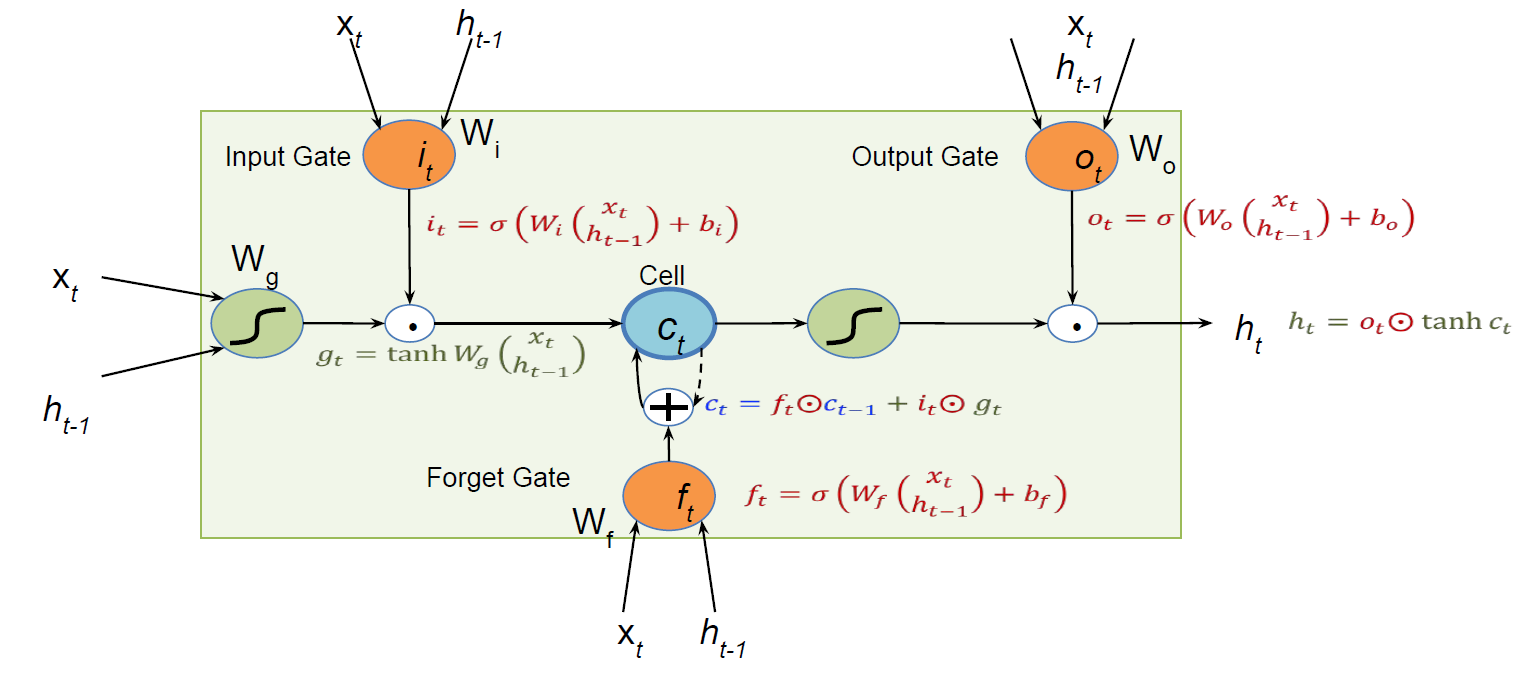
\includegraphics[scale=0.5]{LSTM.PNG}}
\caption{Long-Short Term Memory cell structure and related equations.} % TODO: reference
\label{fig:lstm}
\end{figure*}

The structure of the Long-Short Term Memory cell is shown in Figure \ref{fig:lstm}
and consists of three main gates:

\begin{enumerate}
    \item The \textit{input gate} decides how much input information is added to the current state and is caracterized by the following Equation:
        \begin{equation}
            i_t = \sigma \left(
                W_i
                \begin{pmatrix}
                x_t \\
                h_{t-1}
                \end{pmatrix}
                + b_i
            \right)
        \end{equation}
    
    \item The \textit{forget gate} decides how much of the past should be remembered and is caracterized by the following Equation:
        \begin{equation}
            f_t = \sigma \left(
                W_f
                \begin{pmatrix}
                x_t \\
                h_{t-1}
                \end{pmatrix}
                + b_f
            \right)
        \end{equation}

    \item The \textit{output gate} decides the output based on the current state and is caracterized by the following Equation:
        \begin{equation}
            o_t = \sigma \left(
                W_o
                \begin{pmatrix}
                x_t \\
                h_{t-1}
                \end{pmatrix}
                + b_o
            \right)
        \end{equation}

\end{enumerate}

% The input gate decides how much input information is added to the current state, the 
% forget gate decides how much of the past should be remembered and the output gate 
% decides the output based on the current state.
% The equations

The memory cell $c_t$ is updated as follows:
\begin{equation}
    c_t = f_t \odot c_{t-1} + i_t \odot tanh \left( W_g
        \begin{pmatrix}
            x_t \\
            h_{t-1}
        \end{pmatrix}
        \right) .
\end{equation}

The new hidden state $h_t$ is computed as follows:
\begin{equation}
    h_t = o_t \odot tanh(c_t) .
\end{equation}






\subsection{GRU cell}

\begin{figure}[htbp]
\centerline{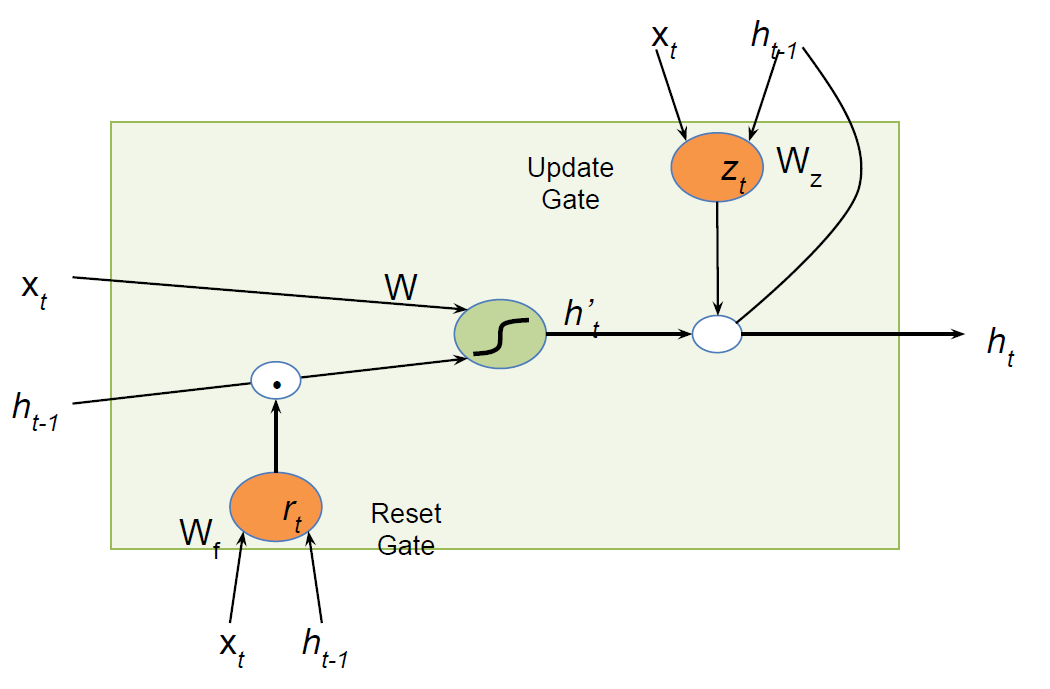
\includegraphics[scale=0.25]{GRU_crop.PNG}}
\caption{Gated Recurrent Unit cell structure.} % TODO: reference
\label{fig:gru}
\end{figure}

The structure of the Gated Recurrent Unit is shown in Figure \ref{fig:gru} 
and consists of two main gates:

\begin{enumerate}
    \item The \textit{reset gate} is used to determine how much of the past 
    information to forget and is caracterized by the following Equation:
        \begin{equation}
            r_t = \sigma \left(
                W_r
                \begin{pmatrix}
                x_t \\
                h_{t-1}
                \end{pmatrix}
                + b_r
            \right)
        \end{equation}
    
    \item The \textit{update gate} helps the model to decide how much of the past 
    information needs to be considered and is caracterized by the following Equation:
        \begin{equation}
            z_t = \sigma \left(
                W_z
                \begin{pmatrix}
                x_t \\
                h_{t-1}
                \end{pmatrix}
                + b_z
            \right)
        \end{equation}

\end{enumerate}

Finally, the new hidden state $h_t$ is computed as follows:
\begin{equation}
    h_t' = tanh \left( W
        \begin{pmatrix}
            x_t \\
            r_t \odot h_{t-1}
        \end{pmatrix}
        \right)
\end{equation}

\begin{equation}
    h_t = (1-z_t) \odot h_{t-1} + z_t \odot h_t'
\end{equation}
